\section{Praktijk: evolutionary improvement}

\subsection{Inleiding}
Nu wij in de vorige hoofdstukken de nodige achterliggende theorie hebben onderzocht, gaan we onze kennis inzetten voor het maken van twee praktijkopdrachten: een spel dat gespeeld moet worden door een zelflerend programma en een zelflerend programma om handgeschreven nummers te herkennen. In dit hoofdstuk zijn wij bezig met de vraag: \textit{welke onderdelen zijn nodig voor een zelflerend computersysteem, in de vorm van een door ons ontworpen computerprogramma, dat in staat is een eenvoudig, zelfgemaakt computerspel, met daarin meerdere obstakels, te spelen?}

\subsection{Het spel}
Voordat we het zelflerende deel van het programma kunnen maken, moet er eerst een spel komen. Hiervoor kiezen wij een \textit{platformer}. Er is een wereld waar de speler doorheen kan springen. Er zitten heuvels, kuilen en gaten in. Wanneer de speler in zo'n gat valt, gaat hij dood. Het doel van het spel is simpelweg zo ver mogelijk te komen. Lopen doe je automatisch, dus het komt echt aan op de timing van je sprong. Voor een mens is dit makkelijk te bevatten, maar voor een computer kan dit een groot obstakel blijken te zijn.
In figuur \ref{fig:platformer1} is goed te zien hoe het spel is opgebouwd uit "blokjes". Op sommige blokjes, de groene, kan de speler staan. Alles wat blauw is, is niet solide en de speler valt er dus doorheen (dit is een eerdere versie van het spel).

\begin{figure}[H]
  \centering
    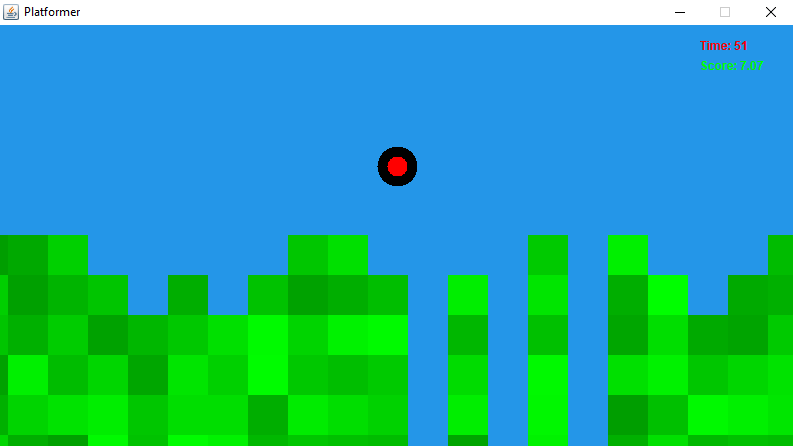
\includegraphics[width=0.5\textwidth]{platformer1.png}
  \caption{De eerste versie van het spel}
  \label{fig:platformer1}
\end{figure}

\subsection{Evolutionary improvement toepassen}
Nu is het tijd om een zelflerend systeem te maken die dit spel kan leren spelen. We doen dit met evolutionary improvement (zie hoofstuk 5). Eigenlijk moet het programma een enkele vraag kunnen beantwoorden: wat is het beste moment om te springen?

Elk individu dat het spel speelt heeft DNA. In dit DNA staat beschreven hoe lang een speler telkens moet wachten voordat hij springt. (Ook staan de kleuren van het blokje en van de ogen hierin beschreven, maar dat heeft geen invloed op het spelen van het spel). Het DNA van de best presterende individuen kan worden doorgegeven tussen generaties. Het idee is dat het programma steeds beter wordt doordat het steeds "beter" DNA voor zijn spelers heeft.
Ook kunnen er willekeurige mutaties en \textbf{crossovers} plaatsvinden. Een mutatie is een willekeurige verandering in het DNA en een crossover is het op twee verschillende plekken wisselen van de informatie op het DNA. Deze acties worden ondernomen om diversiteit in de populatie te vergroten. Stel je voor dat je op tijdstip 4, moet springen, maar geen enkel individu heeft hier de code voor, dan zal er nooit vordering kunnen komen.

De \textit{fitness} van een bepaald individu wordt bepaald door zijn horizontale positie. Komt het individu verder, dan is hij meer geschikt en zal hij dus een hogere fitness hebben. Om tot het getal te komen dat weergegeven wordt als de fitness, wordt de positie echter in het kwadraat gedaan. Dit is niet zonder reden: op het moment dat een bepaald individu w\'el over een gat springt, maar een ander individu niet, dan is het verschil in x-positie niet zo groot, een gat is immers maar 1 of 2 blokjes breed. Om een kleine vooruitgang meer impact te geven op de fitness, kwadrateren we.

\subsection{Het programma}
Zodra je het programma opstart, kan je eerst een keer zelf het spel spelen (springen doe je door op de "w"-toets te drukken). Op het scherm is nu echter een stuk meer te zien dan alleen het spel. Rechtsonder zijn de \textit{Mutation rate} en de \textit{Population size} weergegeven, deze getallen geven respectievelijk aan hoe groot de kans is op een mutatie en de grootte van één generatie aan individuen.

Er zijn ook nog twee knoppen te zien: \textit{Run} en \textit{Run Ten}. Wanneer je op \textit{Run} drukt, maakt het programma \'e\'en generatie individuen aan en laat al deze individuen het spel doorlopen. De generatie staat links weergegeven, op volgorde van hoogste naar laagste fitness. De naamgeving is als volgt: eerst een generatienummer (bijvoorbeeld G10 of G16) en daarna het nummer van het individu uit de generatie (S102, S300, enzovoorts). Als je op een bepaald individu klikt, wordt er afgespeeld hoe hij het spel speelt.

Wanneer je nogmaals op de knop drukt, wordt de volgende generatie aangemaakt. De individuen uit de nieuwe generatie kunnen dus wat DNA "overerven" van de vorige. Links wordt de nieuwe populatie weergegeven. We verwachten hier een hogere fitness te zien, doordat het programma steeds zal proberen het beste DNA door te geven.

Wanneer je op \textit{Run Ten} drukt, loopt de simulatie tien maal en je krijgt de resultaten te zien van de laatste generatie.


\begin{figure}[H]
  \centering
    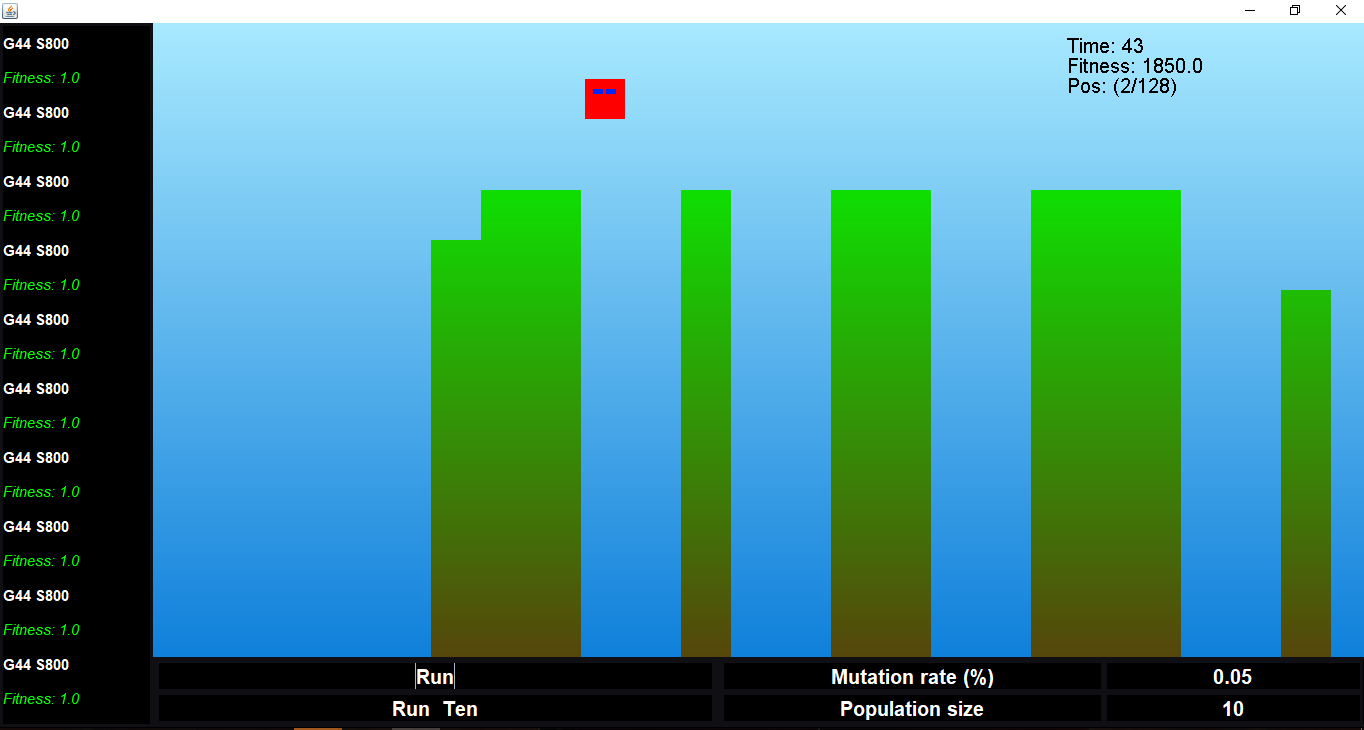
\includegraphics[width=0.5\textwidth]{platformer2.png}
  \caption{Een bepaald individu dat, aangestuurd door het programma, het spel speelt}
  \label{fig:platformer1}
\end{figure}

\subsection{De resultaten}
Het is de bedoeling dat het programma beter wordt in het spelen van het spel, naarmate er meer generaties zijn geweest. En ja hoor! Wanneer je \'e\'en run uitvoert, zie je al een grote verandering in de fitness. Druk je vervolgens nog een aantal keer op \textit{Run Ten}, dan zie je de getallen nog groter worden. In figuur \ref{fig:EvolutionResults} is de fitness te zien van het beste individu van 10 generaties uit 6 verschillende tests (langs de horizontale as staat het generatienummer, langs de verticale staat de fitness). Ook hier is goed te zien dat het programma alsmaar beter wordt. Soms lijkt er generaties lang echter geen vordering te zijn, soms neemt de fitness zelf af, maar vaak komt het programma ook zo'n dipje uit. Dit kan als volgt verklaart worden: het is waarschijnlijk dat er op een bepaalde plek in de wereld, waar de individuen doorheen moeten, een moeilijk obstakel zit, waar nog geen enkel individu het DNA voor heeft om overheen te komen. Nu moet het programma geluk hebben dat er een mutatie plaatsvind, die helpt dit obstakel te overkomen. Bij de rode lijn is bijvoorbeeld te zien dat er rond generatie 80 een daling in fitness plaatsvond, maar ook dat er daarna ook weer vordering kwam.

\begin{figure}[H]
  \centering
    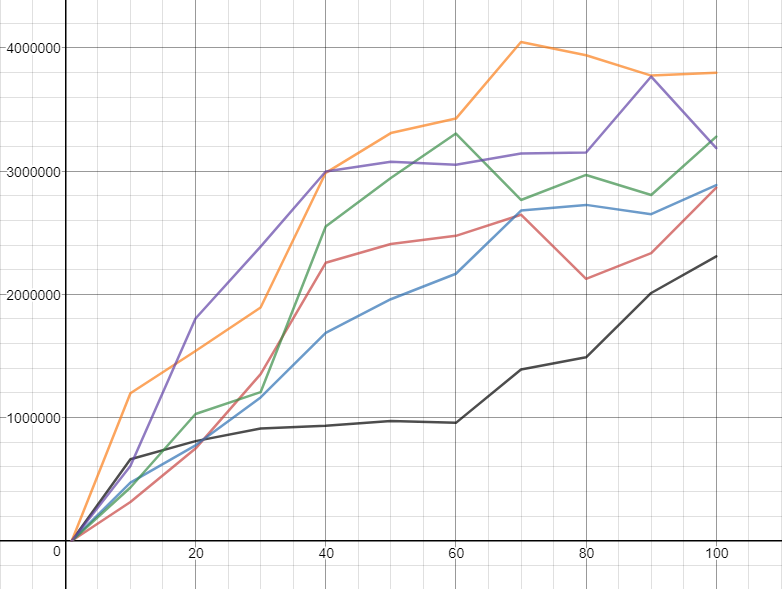
\includegraphics[width=0.7\textwidth]{EvolutionResults.png}
  \caption{De hoogste fitness per 10 generaties voor 6 verschillende tests. Op de x-as staat het aantal generaties, op de y-as staat de hoogste fitness van die generatie. (Grafiek gemaakt m.b.v Desmos \cite{Desmos})}
  \label{fig:EvolutionResults}
\end{figure}

\subsection{Conclusie}
Een computerprogramma blijkt niet erg intelligent te hoeven zijn om zichzelf een spel als deze te kunnen leren spelen. Door middel van willekeurige trial-and-error kan het programma steeds beter worden. Wij hebben gekozen dit evolutionair te doen, maar we denken dat dit ook op de andere in hoofdstuk \ref{chapter:Improvement} genoemde manieren kan. We hebben gemerkt dat de speler, aangestuurd door het programma, zich niet "bewust" hoeft te zijn om de wereld waarin hij loopt, hij hoeft immers alleen te weten wanneer hij over een gat heen moet springen.